\documentclass[supercite]{Experimental_Report}

\title{~~~~~~新生实践课~~~~~~}
\author{陈金岳}
%\coauthor{张三、李四}
\school{计算机科学与技术学院}
\classnum{CS2404}
\stunum{U202414622}
%\costunum{U202115631、U202115631}
\instructor{陈加忠} % 该系列实验报告模板由华科大计院教师陈加忠制作
\date{2024年11月11日}

\usepackage[UTF8,heading = true]{ctex}
\usepackage{algorithm, multirow}
\usepackage{algpseudocode}
\usepackage{amsmath}
\usepackage{amsthm}
\usepackage{framed}
\usepackage{mathtools}
\usepackage{subcaption}
\usepackage{xltxtra} %提供了针对XeTeX的改进并且加入了XeTeX的LOGO, 自动调用xunicode宏包(提供Unicode字符宏)
\usepackage{bm}
\usepackage{tikz}
\usepackage{tikzscale}
\usepackage{pgfplots}
%\usepackage{enumerate}

\pgfplotsset{compat=1.16}

\newcommand{\cfig}[3]{
  \begin{figure}[htb]
    \centering
    \includegraphics[width=#2\textwidth]{images/#1.tikz}
    \caption{#3}
    \label{fig:#1}
  \end{figure}
}

\newcommand{\sfig}[3]{
  \begin{subfigure}[b]{#2\textwidth}
    \includegraphics[width=\textwidth]{images/#1.tikz}
    \caption{#3}
    \label{fig:#1}
  \end{subfigure}
}

\newcommand{\xfig}[3]{
  \begin{figure}[htb]
    \centering
    #3
    \caption{#2}
    \label{fig:#1}
  \end{figure}
}

\newcommand{\rfig}[1]{\autoref{fig:#1}}
\newcommand{\ralg}[1]{\autoref{alg:#1}}
\newcommand{\rthm}[1]{\autoref{thm:#1}}
\newcommand{\rlem}[1]{\autoref{lem:#1}}
\newcommand{\reqn}[1]{\autoref{eqn:#1}}
\newcommand{\rtbl}[1]{\autoref{tbl:#1}}

\algnewcommand\Null{\textsc{null }}
\algnewcommand\algorithmicinput{\textbf{Input:}}
\algnewcommand\Input{\item[\algorithmicinput]}
\algnewcommand\algorithmicoutput{\textbf{Output:}}
\algnewcommand\Output{\item[\algorithmicoutput]}
\algnewcommand\algorithmicbreak{\textbf{break}}
\algnewcommand\Break{\algorithmicbreak}
\algnewcommand\algorithmiccontinue{\textbf{continue}}
\algnewcommand\Continue{\algorithmiccontinue}
\algnewcommand{\LeftCom}[1]{\State $\triangleright$ #1}

\newtheorem{thm}{定理}[section]
\newtheorem{lem}{引理}[section]

\colorlet{shadecolor}{black!15}

\theoremstyle{definition}
\newtheorem{alg}{算法}[section]

\def\thmautorefname~#1\null{定理~#1~\null}
\def\lemautorefname~#1\null{引理~#1~\null}
\def\algautorefname~#1\null{算法~#1~\null}

\begin{document}

\maketitle

\clearpage

\pagenumbering{Roman}

\tableofcontents[level=2]

\clearpage

\pagenumbering{arabic}

\section{网页整体框架}
  	我制作的网页,顶部介绍主题内容,中间正文,在底部有回到主页的超链接文字和图片。提供的选项如下:

\begin{enumerate}
	\renewcommand{\labelenumi}{\theenumi)}
	\item 主页
	\item 个人介绍
	\item 诗文
	\item 游戏
	
\end{enumerate}
\begin{figure}[h] % here top bottom
	\begin{center}
		\includegraphics[scale=0.80]{images/frame.jpg}
		\caption{网站框架}
		\label{fig1-1}
	\end{center}
\end{figure}
	主页的各个选项的解释:\\个人介绍,主要介绍了网页的主要内容,并没有个人资料(保护隐私)。\\诗文,因为比较喜欢苏轼,《定风波》也是我比较喜欢的一首词,所以就把他写在了网页中,来纪念一下这一代鸿儒吧\\游戏,我比较喜欢玩一些剧情游戏,有一种读书般的体验感,剧情所带来的反馈也极为强烈,或是纪念,或是影射,都很有意思,所以姑且提了两嘴。

\section{主页设计}

主页在左上角对访客表示问候,

\begin{figure}[h]
	\begin{center}
		\includegraphics[scale=0.40]{images/first.jpg}
		\caption{主页举例}
		\label{fig2-1}
	\end{center}
\end{figure}

主页的设计如下:选取了一张代表我精神状态的背景图,遇到困难先睡一觉(笑),以养精蓄锐,分别提供了几个选项,分别是个人介绍(readme),诗文(苏东坡《定风波》),游戏,和返回寝室主页。

\newpage

\section{分页面设计}

主要围绕着我个人的各项兴趣爱好展开。

\subsection{个人介绍}

\begin{figure}[h]
	\begin{center}
		\includegraphics[scale=0.20]{images/self.jpg}
		\caption{个人介绍}
		\label{fig3-1}
	\end{center}
\end{figure}
在个人介绍中尽量避免隐私内容,所以我留下了经典款默认签名(不是),简短地介绍了一下网页内容.

\subsection{诗文}

		\includegraphics[scale=0.40]{images/poem.jpg}
		\caption{诗文}
		\label{fig3-2}

在诗文界面,我设计一个文人卡通画作为返回超链接,权当代指苏轼了,然后附上了《定风波》全文和配套赏析。在配图方面,我选了一张苏轼独坐竹林之中,也恰好符合原作中的意境。“莫听穿林打叶生,何妨吟啸且徐行”,“谁怕,一蓑烟雨任平生”这两句也将贯穿我人生的始终。乐天知命也是我所追求的人生境界。

\subsection{游戏}

\begin{figure}[h]
	\begin{center}
		\includegraphics[scale=0.20]{images/game.jpg}
		\caption{游戏}
		\label{fig3-3}
	\end{center}
\end{figure}

我个人比较喜欢玩一些剧情游戏,每次体验这些游戏的时候,都像是经历了一次不同的人生,得到不同的,对现实的感悟和理解,而且,这些游戏带给我的精神上的反馈,都有助于我在现实生活拾起信心。抑或是作为星际游客的开拓精神,抑或是作为一名山间侠盗看尽世态炎凉和人情冷暖,最终奋起反抗,推翻暴政。抑或是创造历史,享受谱写人生的爽快,抑或是见证历史,感受人情世事的厚重和多样。这些带来的新奇体验和经历,也会在网页中体现。

\includegraphics[scale=0.20]{images/laojing.png}
\caption{崩坏星穹铁道}
\label{fig3-3-1}


\includegraphics[scale=0.20]{images/mingmo.png}
\caption{明末千里行}
\label{fig3-3-2}

\subsection{寝室主页}

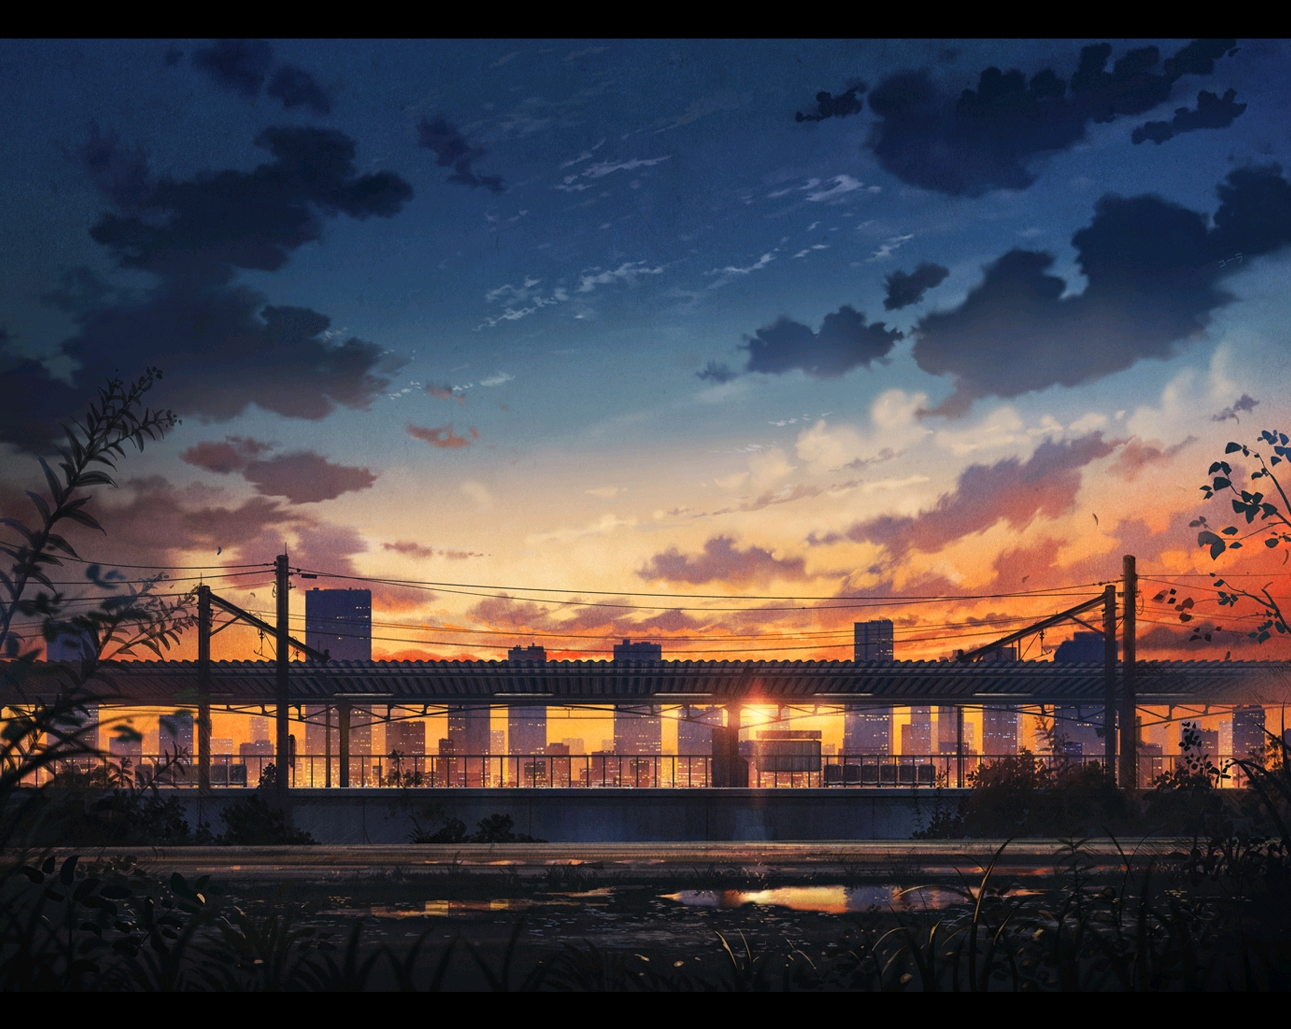
\includegraphics[scale=0.20]{images/qinshi.png}
\caption{寝室主页}
\label{fig3-4}

寝室主页,主要采用了flexbox的设计方式,使四个qq头像居中均分,作为链接各个网页的超链接选项,背景图选了一个热门壁纸,还挺好看。

\newpage

\section{网页设计小结}

在网页的设计中,确实遇到了很多问题,比如,我想在主网页的设计中使变换按钮更加人性化(也就是以按钮的形式体现),但是我在dw中并没有发现这个画图的功能,于是我下载了ps,将自己的图片导入后,进行编辑,插入了几个图层,形成按钮,并且了解了一些快捷键的使用,现在已经能借助ps对图片进行小小的改动了,也算是解决问题之后的一点小收获了。

再然后我苦于单调无味的白色背景,我在仔细研究之后发现了css中设置背景的功能,于是我欢天喜地地添加了一张自己喜欢的图片进去,然后返回拆分界面时,不仅背景不居中,而且重影。我上网查了一些资料,补充了一些有关背景的代码,才让背景顺着自己的心意达到全网页覆盖的效果(因为网页内容没那么多也不需要翻页)。

\newpage

\section{课程的收获和建议}

课程收获很多,恶补了之前比较稀松的计算机知识,并且区分了很多计算机的概念和操作方法,广泛地了解了有关计算机的几种工具,也了解了例如Python这样热门的编程语言,主要还是激发了兴趣,让我知道学了计算机都能干些什么。

\subsection{计算机基础知识}

在第一节课的时候,以往成长在书本中的我确实被各种计算机知识深深吸引,我觉得特别有意思的一段就是教授我们如何配一台自己的台式机的时候,二手的性价比在陈老师的口中可谓无上之选,老师提供的各种软件(特指winrar)确实很好用。建议明年陈老师在讲配台式的时候压缩预算,吧主机外壳换成纸壳()。

\subsection{文档撰写工具LaTeX}

latex为我带来了除了word之外另一种编写报告的方式,它的排版整洁,相比word的容易错版,依托这个模板,它能使我的报告看起来更加赏心悦目,并且在配置的过程中也让我了解了多种获取资料的方式。


\subsection{编程工具Python}

收获:对装解释器,了解python的基本结构和框架有了一些了解。并且了解了一些基本的类型。计算思维这门课程也需要python,也算是入了门吧。
建议:建议老师明年可以在“类”的讲解上稍微多花一些时间,之前刚学的时候确实有一些云里雾里。。。

\subsection{图像设计软件Photoshop}

这个学期没有这个,但是要完成网页设计也确实少不了这个,收获一些比较基础的操作吧算是。

\subsection{版本管理软件Git}

收获:之前在学校社团面试的时候就要求对git有了解,这次新生实践课上也实际去操作了,发现了以前学习时没有发现的问题,对我之后的小组作业会有很大帮助。
建议:可以多介绍几种命令行(?

\subsection{网页制作Dreamweaver}

接触Dreamweaver,确实为我打开了新世界的大门,让我初步了解了前端工作者的工作,激发了我对前端的浓厚兴趣。
收获:了解了如何初步使用Dreamweaver,设计自己的网页,初步了解了如何布局网页。

%\nocite{*} %% 作用是不对文献进行引用,但可以生成文献列表

%\bibliographystyle{Experimental_Report}
%\bibliography{Experimental_Report}
%\setcounter{secnumdepth}{0}
%\appendix

%\section{附录A 功能模块一实现的主要源程序}

%\noindent
%/* Linear Table On Sequence Structure */\\
%\#include <stdio.h>\\
%\#include <malloc.h>\\
%\#include <stdlib.h>\\

%\noindent
%/*---------page 10 on textbook ---------*/\\
%\#define TRUE 1\\
%\#define FALSE 0\\
%\#define OK 1\\
%\#define ERROR 0\\
%\#define INFEASTABLE -1\\
%\#define OVERFLOW -2\\
%\newpage
%\section{附录B 功能模块二实现的主要源程序}
%\newpage
%\section{附录C 功能模块三实现的主要源程序}
%\newpage
%\section{附录D 功能模块四实现的主要源程序}

\end{document}